%!TEX root = ../nwoods_thesis.tex

\chapter{Analysis Strategy}\label{ch:methods}

\section{Background Estimation}\label{sec:bkg}
Reducible backgrounds for four-lepton events typically have two or three prompt leptons and two or one other objects---typically jet fragments, sometimes photons---which are misidentified as prompt leptons.
The largest source of background contamination is from events in which a {\PZ} boson is produced in association with a photon and a jet, a leptonically-decaying $\PW$ boson and a jet, or two jets.
There is also a contribution from {\TTbar} events in which both top quarks decay to a lepton, a neutrino, and a {\Pqb}~quark jet.
For simplicity, the two sets of processes are not treated separately in what follows, and are collectively labeled ``$\PZ+\PX$'' events\footnote{This is a bit of a misnomer, as ``$\PZ+\PX$'' does not accurately describe {\TTbar} events, but the terminology is retained here for consistency with the CMS papers on these analyses.}.

The contributions of the reducible backgrounds to the selected four-lepton signal samples are evaluated using the tight-to-loose ``fake rates'' method, described in Ref.~\cite{Chatrchyan:2013mxa}.
In this procedure, the likelihood of a nonprompt (``fake'') object to be misidentified as a prompt lepton is estimated and applied to control regions enriched with $\PZ+\PX$ events to estimate their contribution to the signal region.
The lepton misidentification rate $f_\ell\left(\pt^\ell, \eta^\ell\right)$ is measured from a sample of $\PZ + \ell_\text{fake}$ events, where the {\PZ} boson candidate is selected as in the signal region but with $\left| m_{\ell\ell} - m_\PZ \right| < 10\GeV$, and the $\ell_\text{fake}$ object is a lepton candidate that passes relaxed ID requirements as defined in Section~\ref{sec:looseID}, with no isolation or tight ID requirements applied.

The misidentification rate is defined as the fraction of $\ell_\text{fake}$ candidates which pass full lepton identification and isolation critera, in bins of $\pt$ and $\eta$.
One should note that the misidentification rate cannot be interpreted as a probability in the usual sense, and if fact there is no simple physical interpretation of it.
Events with three prompt leptons can contaminate this control region and bias the misidentification rate, because the {non-\PZ} lepton is falsely assumed fake.
To mitigate this bias, the $\WZ \to 3\ell\nu$ yields in the numerator and denominator in each bin are estimated from a simulated sample and subtracted before the ratio of yields is taken.
Figure~\ref{fig:fakerates} shows the misidentification rates for electrons and muons separately as a function of {\pt} and $\eta$.

\begin{figure}[htbp]
  \begin{center}
    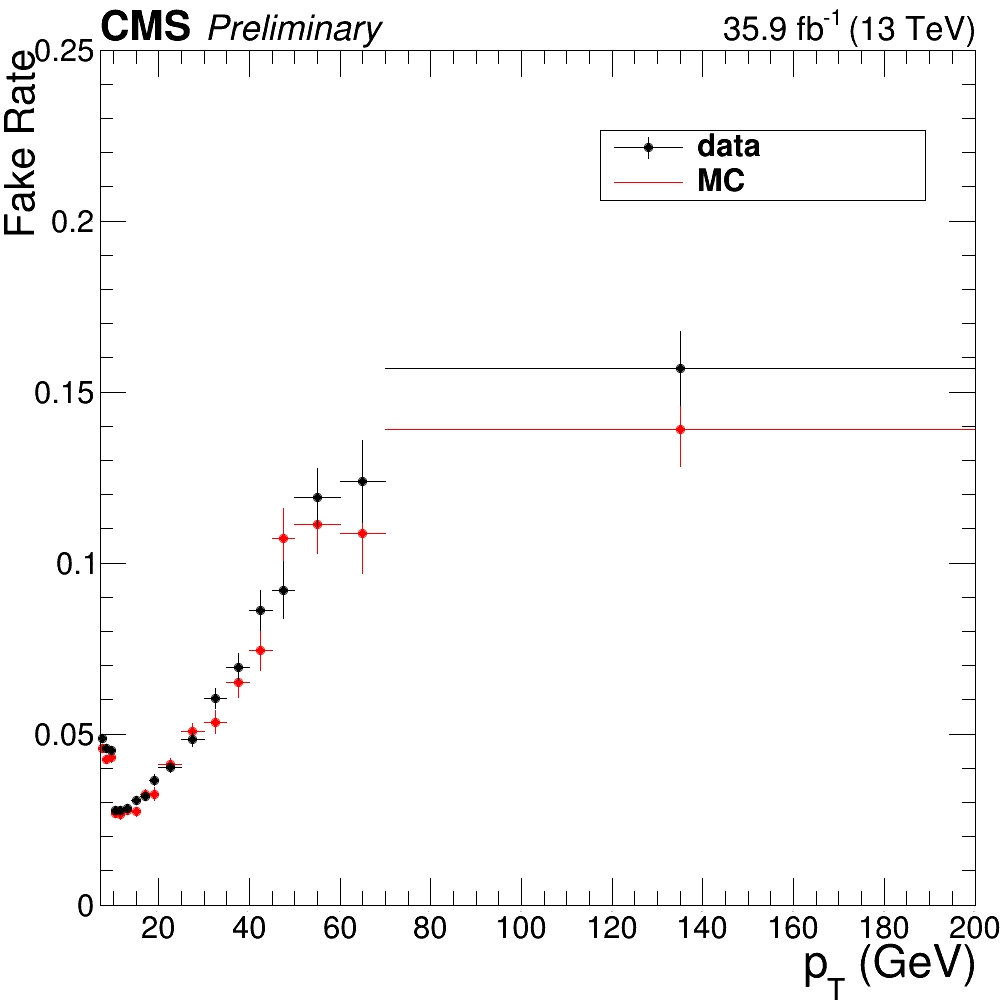
\includegraphics[width=0.35\textwidth]{methods/eFakeRate_pt.png}
    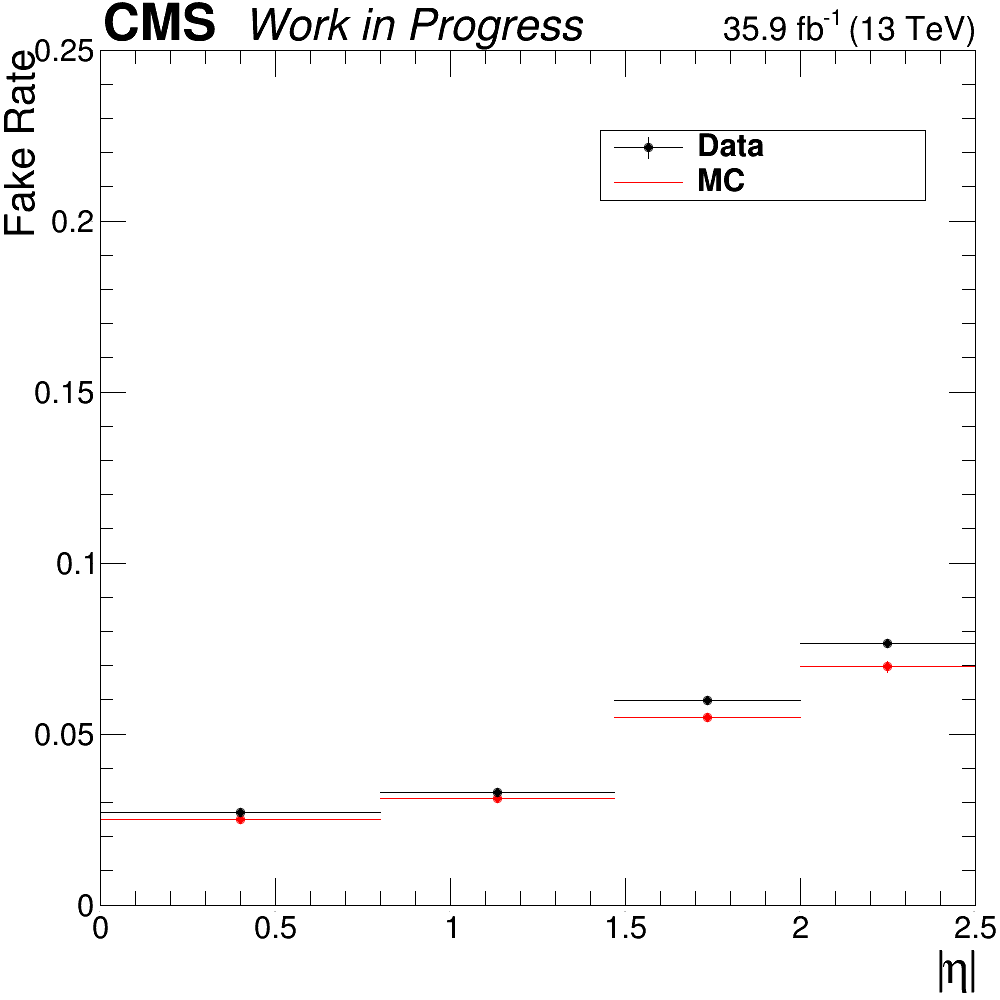
\includegraphics[width=0.35\textwidth]{methods/eFakeRate_eta.png} \\
    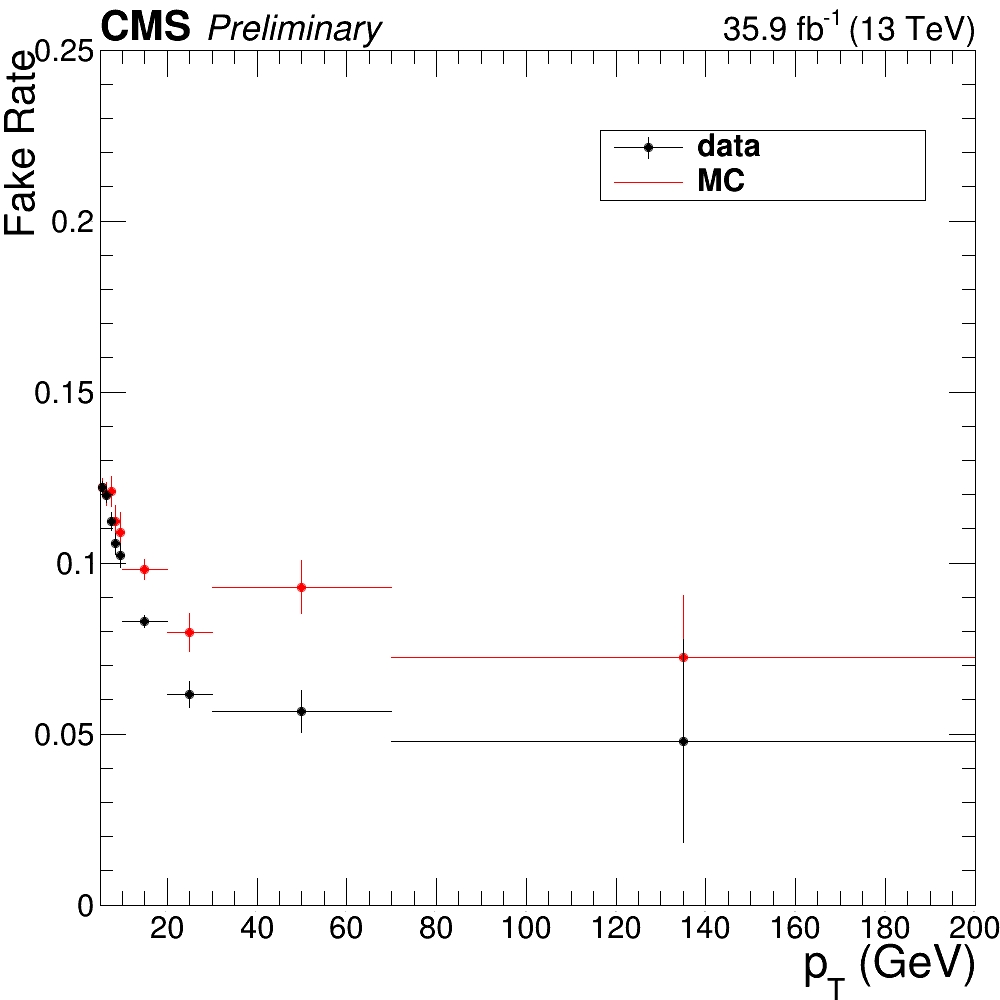
\includegraphics[width=0.35\textwidth]{methods/mFakeRate_pt.png}
    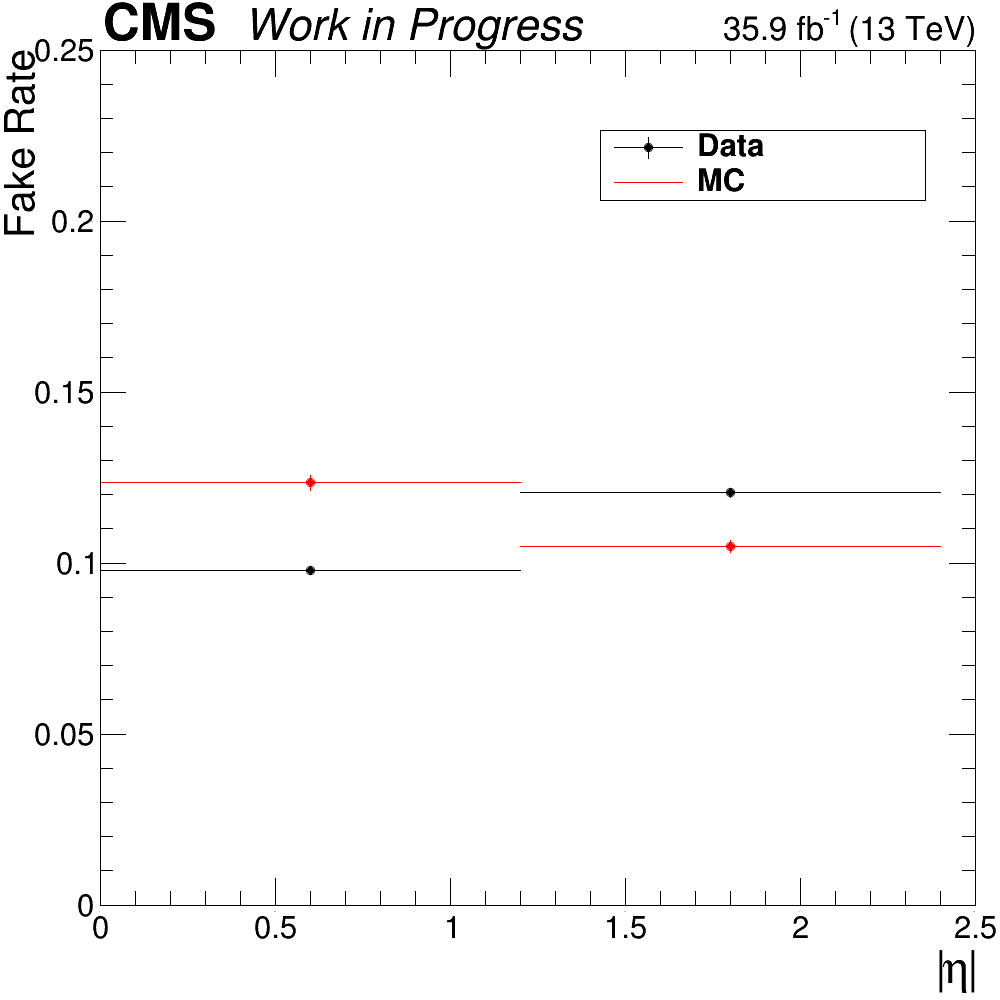
\includegraphics[width=0.35\textwidth]{methods/mFakeRate_eta.png}
    \caption[Misidentification rates for electrons and muons]{
      Fake rate for electrons~(top) and muons~(bottom) as a function of $\pt$~(left) and $\eta$~(right).
      }\label{fig:fakerates}
  \end{center}
\end{figure}

To estimate the total reducible background yield, the misidentification rates are applied to two $\PZ+\PX$ enriched control samples, each containing a {\PZ}~boson candidate passing all signal region requirements plus two more lepton candidates which pass the relaxed identification criteria and would make a second {\PZ} boson candidate according to Section~\ref{sec:zSelection} except that one or both fail the full identification or isolation criteria.
The sample with one failing lepton, called the ``3P1F'' sample for ``3 prompt 1 fake,'' covers the contribution from {\WZ} events, while the sample with both leptons in the second {\PZ} boson failing (``2P2F'') covers $\PZ+\text{jets}$ and {\TTbar} events.
The fake object transfer factor
\begin{equation}
  F_\ell\left(\pt^\ell,\eta^\ell\right) = \frac{f_\ell\left(\pt^\ell, \eta^\ell\right)}{1 - f_\ell\left(\pt^\ell, \eta^\ell\right)}
\end{equation}
is the ratio of nonprompt objects passing the relaxed and full selection criteria, and thus serves as a per-lepton extrapolation factor between control sample yields and signal sample yields.

The total reducible background yield is thus
\begin{equation}\label{eq:bkgYield}
  N_\text{bkg} = \sum_{\ell \in \text{3P1F}} \! \! F_\ell\left(\pt^\ell,\eta^\ell\right) - \! \! \! \! \! \! \sum_{\ell_1,\ell_2 \in 2P2F} \! \! \! \! \! F_{\ell_1}\left(\pt^{\ell_1},\eta^{\ell_1}\right)F_{\ell_2}\left(\pt^{\ell_2},\eta^{\ell_2}\right).
\end{equation}
The minus sign prevents double-counting of $\PZ+2\text{jets}$ events in which one jet fragment is misidentified.
The failing lepton candidates in the 3P1F and 2P2F control samples are assumed to truly be jet fragments or other nonprompt objects, but selection inefficiencies may cause prompt leptons to fail and contaminate the control regions with signal events.
The yield of such signal events in the backgound control regions is estimated by applying the same fake factors to failing events in the {\ZZ} signal Monte Carlo samples, and subtracted from the result of Eq.~(\ref{eq:bkgYield}).

There are also irreducible background contributions from {\TTZ} and {\WWZ} events, which can have four prompt leptons.
Expected yields for these processes are taken from simulation.



\section{Systematic Uncertainties}

Systematic uncertainties for trigger efficiency are taken to be the difference between trigger efficiencies in data and in simulated signal events, found to be around 2\% of the final event yield.
Because leptons in $\PZ \to 4\ell$ events generally have lower $\pt$, the uncertainty increases to 4\% for $\PZ \to 4\Pe$ events.
In both data and simulated events, trigger efficiencies are found with a tag-and-probe technique~\cite{CMS:2011aa}, performed on four-lepton events.

The lepton identification and isolation efficiencies in simulation are corrected with scaling factors derived with the tag-and-probe method, performed on $\PZ \to \ell^+\ell^-$ events in data and a {single-\PZ} Monte Carlo sample.
To find the uncertainties associated with these corrections, the total yield is recomputed with the scaling factors varied up and down by one standard deviation of the uncertainties from the tag-and-probe method, treating all bins as correlated.
The resulting changes in the $\ZZ \to 4\ell$ yield, taken to be the one sigma variations resulting from lepton efficiency uncertainties, are found to be 6\% in the $4\Pe$ final state, 3\% in the $2\Pe2\Pm$ final state, and 2\% in the $4\Pm$ final state.
Leptons in $\PZ \to 4\ell$ events tend to have lower {\pt}, and the tag-and-probe samples for leptons with {\pt} below about {15\GeV} are smaller and more contaminated with nonprompt objects, so the uncertainties are larger; they are found to be 10\%, 6\%, and 7\% for the $4\Pe$, $2\Pe\Pm$, and $4\Pm$ final states, respectively.

The uncertainty on the integrated luminosity of the data sample is 2.5\%~\cite{CMS-PAS-LUM-17-001}.

The uncertainty on lepton fake rates is 40\%, which includes both statistical uncertainty and systematic uncertainties associated with the loosened lepton selections defined in Section~\ref{sec:looseID} and the differences in the underlying physics processes between events in the $\PZ + \ell_\text{fake}$, 3P1F, and 2P2F control samples~\cite{CMS:2014xja}.
Statistical uncertainties arising from the limited size of the $\PZ+\PX$ control samples are also included as a systematic uncertainty on the background yield.
The total uncertainty on the background yield varies by channel but is below 1\% of the expected total yield.

Uncertainties due to the effect of QCD scale on the $\ZZ \to 4\ell$ acceptance are evaluated with {\POWHEG} and {\MCFM}, by varying the QCD scales up and down by a factor of two with respect to the default $\mu_R = \mu_F = m_{\ZZ}$.
Parametric  uncertainties (PDF$+ \alpha_s$) are evaluated according to the \textsc{pdf4lhc} prescription in the acceptance calculation~\cite{Butterworth:2015oua}, and with \textsc{nnpdf3.0} in the cross section calculations.
An additional theoretical uncertainty arises from scaling the $\Pq\Paq \to \ZZ$ and $\Pg\Pg \to \ZZ$ simulated samples to their NNLO and NLO predicted cross sections, respectively, with the $K$~factors described in Section~\ref{sec:samples}.
The corresponding change in the acceptance, 1.1\%, is added to the previous theoretical errors in quadrature.

Systematic uncertainties on expected signal yield are summarized in Table~\ref{tab:systematics}.
To obtain uncertainties in the inclusive cross sections, each uncertainty source is treated as a nuisance parameter in the fits described in Section~\ref{sec:signalStrength}.
For differential cross section and other shape uncertainties, the calculation  is fully redone for each uncertainty source, with the inputs shifted by one standard deviation in each direction.
Variations across bins are taken to be fully correlated for each uncertainty source.
Lepton and jet momentum scale and resolution uncertainties are taken to be trivial for the overall yield, but they are considered among the shape uncertainties.

\begin{table}[htbp]
  \centering
  \caption[Systematic uncertainties on the total yield]{
    The contributions of each source of signal systematic uncertainty in the total yields.
    The integrated luminosity uncertainty and the PDF and scale     uncertainties are considered separately.
    All other uncertainties are added in quadrature into a single systematic uncertainty.
    Uncertainties that vary by decay channel are listed as a range.
  }\label{tab:systematics}
  \begin{tabular}{lcc}
    \toprule
    Uncertainty               & $\PZ  \to  4\ell$ & $\ZZ  \to  4\ell$  \\
    \midrule
    Lepton efficiency         & 6--10\%           & 2--6\%             \\
    Trigger efficiency        & 2--4\%            & 2\%                \\
    MC statistics             & 1--2\%            & 0.5\%              \\
    Background                & 0.6--1.3\%        & 0.5--1\%           \\
    Pileup                    & 1--2\%            & 1\%                \\
    \midrule
    PDF                       & 1\%               & 1\%                \\
    QCD Scales                & 1\%               & 1\%                \\
    \midrule
    Integrated luminosity     & 2.5\%             & 2.5\%              \\
    \bottomrule
  \end{tabular}
\end{table}



\section{Fiducial and Total Cross Section Calculation}\label{sec:xSecCalc}

Inclusive cross section measurements can be treated as simple binned counting experiments, where the bins are the three decay channels ($4\Pe, 2\Pe2\Pm$, and $4\Pm$).
If $\nu$ events are expected in a given bin, the probability of observing $n$ events is given by the Poisson distribution,
\begin{equation}\label{eq:poisson}
  f\left(n; \nu\right) = e^{-\nu}\frac{\nu^{n}}{n!}.
\end{equation}
In a particle physics analysis like this one, $\nu$ takes the form
\begin{equation}\label{eq:expectedYield}
  \nu = \nu_s\left(\nuisS\right) + \nu_b\left(\nuisB\right) = \mu\left(\nuisS\right) \lumiL_\textit{int} \sigma_\textit{SM} \epsilon + \nu_b\left(\nuisB\right)
\end{equation}
where $\nu_s$ and $\nu_b$ are respectively the expected signal and background yields, $\sigma_\textit{SM}$ is the standard model expectation for the cross section of the signal process and $\epsilon$ is our efficiency for detecting and identifying its events.
The signal and background nuisance parameter vectors $\nuisS$ and $\nuisB$ represent hidden quantities that we do not measure directly but which affect our yields, i.e.\ systematic effects.
The signal strength $\mu$ compares our expectation to what we actually measure:
\begin{equation}\label{eq:signalStrength}
  \mu = \frac{\sigma_\textit{meas}}{\sigma_\textit{SM}}.
\end{equation}

Of the variables in Eqs.~(\ref{eq:poisson}) and~(\ref{eq:expectedYield}),  $\sigma_\textit{SM}$ is known from theoretical calculations, and $\epsilon$ is determined from simulation.
The CMS detector is designed to measure $n$ and $\lumiL_\textit{int}$, $\nu_b$ is estimated from data or simulation, and inferring $\sigma_\textit{meas}$ is a matter of finding the most likely value of the signal strength $\mu$ given the observed data.
Then the measured cross section is simply
\begin{equation}\label{eq:xsecCalculation}
  \sigma_\textit{meas} = \mu\sigma_\textit{SM}.
\end{equation}
One interesting feature of this method is that $\sigma_\textit{SM}$ is used in the calculation of $\mu$ (Eq.~(\ref{eq:expectedYield})) and in the final cross section (Eq.~(\ref{eq:xsecCalculation})) in such a way that it cancels out, and in fact anything proportional to the true cross section may be used.
In practice, this means that the order at which $\sigma_\textit{SM}$ is calculated does not matter to the extent that higher order corrections to the kinematics of the events do not affect $\epsilon$.

Typically, $\sigma_\textit{meas}$ in Eq.~(\ref{eq:xsecCalculation}) is the fiducial cross section, the cross section  for the process in a phase space similar to (typically, slightly larger than) the phase space in which the experimental analysis can in principle detect events.
In the four-lepton case, the fiducial phase space is a space of $2\ell2\ell' \left(\ell, \ell' \in \Pe, \Pm\right)$ events defined by criteria on lepton kinematics, dilepton invariant masses, and four-lepton mass.
Table~\ref{tab:fiducialDefs} shows the fiducial definitions for both the $\PZ \to 4\ell$ and $\ZZ \to 4\ell$ cross section measurements.
Lepton kinematic requirements and an invariant mass requirement on all opposite-sign, same-flavor lepton pairs in the event are common to both measurements; requirements on the invariant masses of {\Zgs} boson candidates and the four-lepton system are different.

The total {\ZZ} cross section is defined subject to no constraints except the requirement that $m_{\PZ_1}$ and $m_{\PZ_2}$ be between 60 and 120\GeV, which serves as the definition of a $\PZ$ boson.
The fiducial cross section is related to the total cross section by the branching fraction $\mathcal{B}$ to the final state in question---here, two factors of the {\Zgs} branching ratio to electron and muon pairs---and an acceptance factor $\mathcal{A}$ which is the fraction of events falling in the fiducial phase space,
\begin{equation}\label{eq:fidToTot}
  \sigma_\mathit{fid} = \mathcal{A} \sigma_\mathit{tot} \left( \mathcal{B}\left(\PZ \to 2\ell\right) \right)^2.
\end{equation}
The acceptance factor $\mathcal{A}$ is determined entirely from theory, and is well known~\cite{Olive:2016xmw}, so it is straightforward to calculate the total cross section once the fiducial cross section is known.
Calculating both fiducial and total cross sections is interesting because it effectively factorizes experimental and theoretical uncertainties.
The experimental uncertainties are contained entirely in the uncertainties on $\epsilon$, $\lumiL_\textit{int}$, and $\nu_b$ in Eq.~(\ref{eq:expectedYield}), which have little or no dependence on theory, while the theoretical uncertainties are contained entirely in the uncertainty on $\mathcal{A}$, which is determined with no experimental input.
Thus the uncertainty on $\sigma_\textit{fid}$ is entirely experimental, and the theoretical uncertainties enter only in the uncertainty on $\sigma_\textit{tot}$.

\begin{table}[htbp]
  \centering
  \caption[Fiducial phase space definitions]{
    Fiducial phase space definitions for the $\PZ \to 4\ell$ and $\ZZ \to 4\ell$ cross section measurements.
    The common requirements apply to both.
    The $m_{\ell^+\ell^{\prime -}}$ criterion is applied to all opposite-sign same-flavor lepton pairs in the event.
  }\label{tab:fiducialDefs}
  \begin{tabular}{ll}
    \toprule
    Measurement       & Fiducial requirements                             \\
    \midrule
    Common            &  $\pt^{\ell_1} > 20\GeV$, $\pt^{\ell_2} > 10\GeV$, $\pt^{\ell_{3,4}} > 5\GeV$,                                       \\
                      & $\abs{\eta^{\ell}} < 2.5$, $m_{\ell^+\ell^-} > 4\GeV$                                          \\
    \midrule
    $\PZ \to 4\ell$   & $m_{\PZ_1} > 40\GeV$, $80 < m_{4\ell} < 100\GeV$  \\
    \midrule
    $\ZZ \to 4\ell$   & $60 < m_{\PZ_1},m_{\PZ_2} < 120\GeV$              \\
    \bottomrule
  \end{tabular}
\end{table}


\subsection{Signal Strength Extraction}\label{sec:signalStrength}

The signal strength is found by the method of maximum likelihood~\cite{Olive:2016xmw,bohm2010introduction}.
The likelihood function is the product of the probability distributions across all bins,
\begin{equation}
  L\left(\nuisS,\nuisB\right) = \prod_\textit{bins} f\left(n; \nu\left(\nuisS,\nuisB\right) \right).
\end{equation}
The most likely value of $\nu$ is the one that maximizes $L$.
In practice, $\log L$ is typically maximized instead because it is easier to work with,
\begin{equation}
  \frac{\partial^2 \log L}{\partial \nuisS \partial \nuisB} = 0.
\end{equation}
This maximization is performed simultaneously for all bins, yielding a single signal strength across all channels.
Systematic uncertainties enter as log-normal constraints imposed on the fit, encoded in $\nuisS$ and $\nuisB$.
The fit is performed numerically.


\subsection{\texorpdfstring{$\mathrm{Z} \to 4\ell$}{Z to 4l} Branching Fraction}

The total {\PZ} cross section can be calculated from the $\PZ \to 4\ell$ fiducial cross section with Eq.~(\ref{eq:fidToTot}), but it is better measured in the $2\ell$ channel, where the larger branching fraction yields samples several orders of magnitude larger than the $\PZ \to 4\ell$ sample used here.
It is therefore more interesting to use $\sigma_\textit{fid}\left(\PZ \to 4\ell\right)$ for a measurement of the four-lepton branching fraction $\mathcal{B}\left(\PZ \to 4\ell\right)$.
After applying the acceptance correction to obtain $\sigma_\textit{tot} \left(\PZ \to 4\ell\right) = \sigma_\textit{fid}\left(\PZ \to 4\ell\right) / \mathcal{A}$, the four-lepton branching fraction is given by
\begin{equation}\label{eq:brCalc}
  \mathcal{B}\left(\PZ \to 4\ell\right) = \frac{\sigma_\textit{tot} \left(\PZ \to 4\ell\right)} {\mathcal{C}^{\text{60--120}}_{\text{80--100}} \, \sigma \left(\PZ \to 2\ell\right)}\mathcal{B}\left(\PZ \to 2\ell\right),
\end{equation}
where $\sigma \left(\PZ \to 2\ell\right)$ is the dileptonic {\PZ} cross section in the {60--120\GeV} mass range and $\mathcal{C}^{\text{60--120}}_{\text{80--100}}$ corrects for the fact that $\sigma\left(\PZ \to 4\ell\right)$ is found in a mass range of {80--100\GeV}.



\section{Differential Cross Sections}\label{sec:diffXSec}

Measurement of a differential fiducial cross section is also a problem of finding the most likely true distribution given observed yields in multiple bins, estimated background yields, and detector effects understood through simulation.
Unlike the inclusive cross section, however, finite detector resolution leads to ``smearing'' effects that cause events to migrate across bins, in addition to the same inefficiencies.
The mean detector-level distribution $\vec{\delta}$ is related to the true distribution $\vec{\theta}$ by a response matrix $\mathbf{R}$:
\begin{equation}
  \vec{\delta} = \mathbf{R}\vec{\theta}.
\end{equation}
The observed distribution in data $\vec{d}$ is sampled from the Poisson distribution with mean $\vec{\delta}$ independently in each bin.
CMS simulation software is sufficiently sophisticated to give a good estimate of $R$, reproducing the real detector's resolution and smearing effects at the level of a few per cent or better for all distributions of interest.

If $\mathbf{R}$ is square and invertible, the maximum likelihood estimate (MLE) of the true distribution, $\hat{\vec{\theta}}$, is given by
\begin{equation}\label{eq:unfoldingMLE}
  \hat{\vec{\theta}} = \mathbf{R}^{-1}\vec{d}.
\end{equation}
Even when $\mathbf{R}$ is invertible, however, it is frequently ill-conditioned, giving $\hat{\vec{\theta}}$ unphysical features like large bin-by-bin fluctuations or even negative bins as a consequence of the stochastic nature of $\vec{d}$.
It is therefore necessary to use a more sophisticated procedure to ensure the differential cross section distributions obey physics-inspired constraints.
The variables used for differential cross sections in this analysis are in general well-measured, so bin-to-bin fluctuations are small and the response matrices are nearly diagonal, but some bins have low occupancy which can still cause pathologies.

\subsection{Unfolding}\label{sec:unfolding}

The technique used here is an iterative frequentist method developed in high energy physics by D'Agostini~\cite{DAgostini:1994fjx} and independently in other fields~\cite{Dempster:10.2307/2984875,Lucy:1974AJ,Richardson:72,Shepp:4307558}, as implemented in \textsc{RooUnfold}~\cite{Adye:2011gm}.
At iteration $k$, bin $j$ of the predicted true distribution is set based on its expected contribution to all other bins, weighted by the observed data yield in each:
\begin{equation}
  \begin{split}
    \theta_j^{(k+1)} & = \sum_i \mathbf{R}_{ij} \theta_j^{(k)} \frac{d_i}{\delta_i} \\
    & = \sum_i \mathbf{R}_{ij} \theta_j^{(k)} \frac{d_i}{\sum_m \mathbf{R}_{im} \theta_m^{(k)}}.
  \end{split}
\end{equation}
After several iterations, $\vec{\theta}^{(k)}$ depends only weakly on the ansatz $\vec{\theta}^{(0)}$.

The sequence will converge to the MLE for any non-pathological choice of $\vec{\theta}^{(0)}$~\cite{vardi1985} but again the MLE often displays unphysical behavior.
If $\vec{\theta}^{(0)}$ is strictly positive, $\vec{\theta}^{(k)}$ will be strictly positive for all $k$, and in this case $\hat{\vec{\theta}}$ (as defined in Eq.~(\ref{eq:unfoldingMLE})) will be the asymptotic unfolded distribution as long as it is also strictly positive.
Choosing a smooth function for $\vec{\theta}^{(0)}$ will generally lead to smooth $\vec{\theta}^{(k)}$ for small $k$; typical choises include a flat initial distribution and the truth-level distribution used to construct $\mathbf{R}$ (used in this analysis).
What constitutes ``small'' $k$ depends on the condition of $\mathbf{R}$, but for most physics distributions of interest, including all those used in this analysis, nonphysical fluctuations do not arise until after $\vec{\theta}^{(k)}$ is close to convergence.
Full regularization is therefore imposed by ceasing iteration early.
For all distributions shown here, stopping after four iterations was found to obtain a result close to the asymptotic distribution without artificially increasing the bin-to-bin variance.

\subsection{Uncertainties}

The largest uncertainties in the unfolded distributions arise from the unfolding procedure itself, which can inflate statistical uncertainties present in the detector-level distributions.
The correlation matrix which gives the full uncertainty---considered the statistical uncertainty of the unfolded distribution---does not have a closed form due to the nonlinearity of the method.
The covariance matrix is therefore estimated by propagating the statistical error of the inputs at each iteration of the method, as laid out in Ref.~\cite{DAgostini:1994fjx} and improved in Ref.~\cite{Adye:2011gm}.
This procedure does not account for the bias introduced by regularization, but this is expected to be negligible relative to other systematic uncertainties for the well-modeled processes studied here.

Most systematic uncertainties are propagated through unfolding by recomputing the response matrix with the training sample shifted or reweighted to reflect a $1\sigma$ shift in the quantity in question.
The uncertainty related to that quantity is taken to be the resulting shape difference in the final unfolded distribution.
Systematic uncertainties are negligible compared to statistical uncertainties in most bins, as seen in Fig.~\ref{fig:unfold_unc}, which shows the sources of shape uncertainties on the normalized differential cross section as a function of four-lepton invariant mass.

\begin{figure}[htbp]
  \begin{center}
    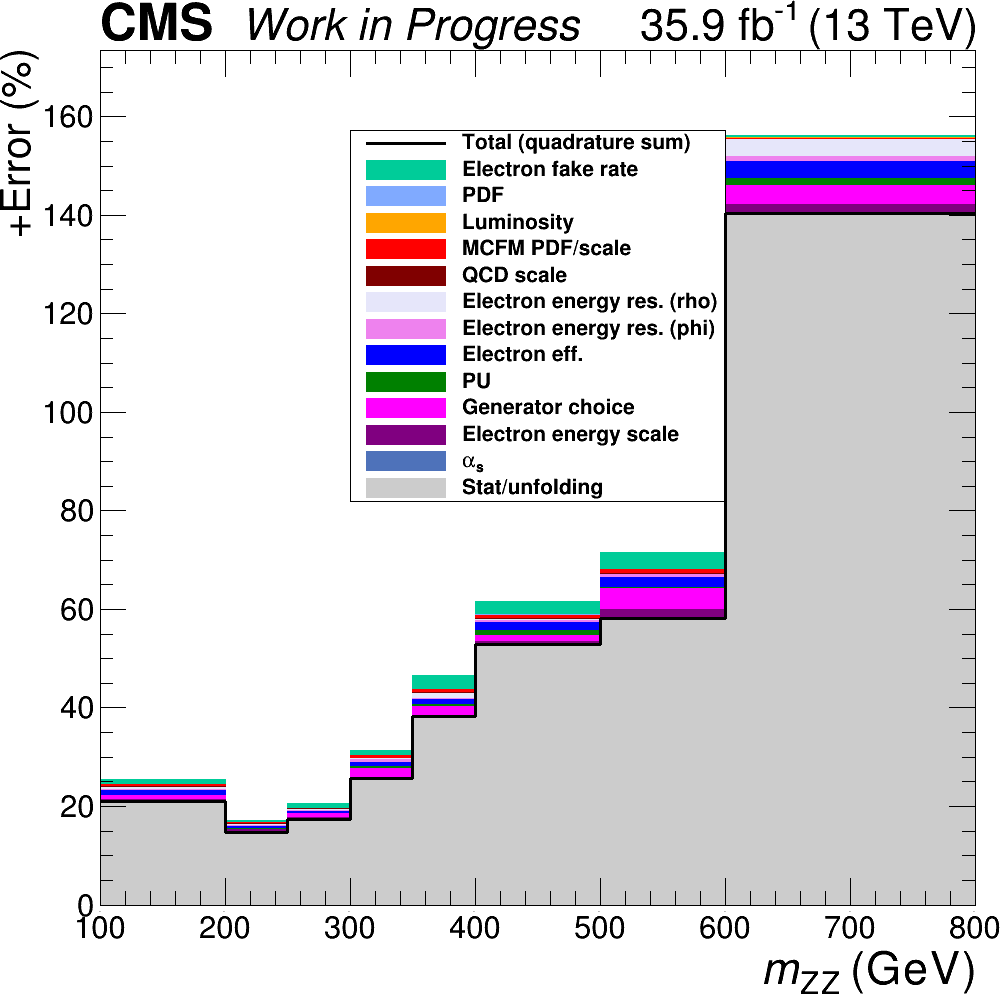
\includegraphics[width=0.45\textwidth]{methods/errUp_mass_eeee.png}
    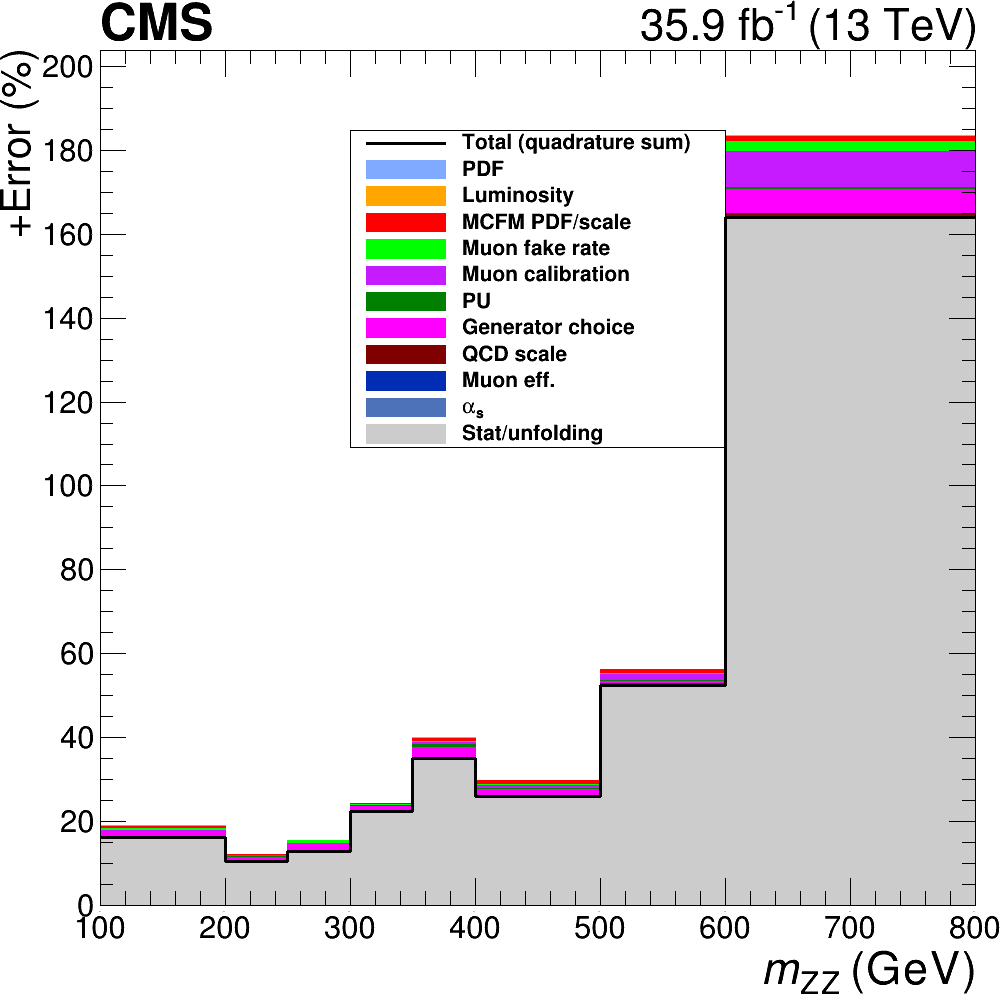
\includegraphics[width=0.45\textwidth]{methods/errUp_mass_mmmm.png}
    \caption[Differential cross section shape uncertainty sources]{
      Sources of positive shape uncertainties for the normalized differential cross section as a function of four-lepton mass, for $4\Pe$ events (left) and $4\Pm$ events (right).
      The grey histogram represents statistical errors, propagated through the unfolding procedure, and the histograms stacked on top of it represent various sources of systematic uncertainty.
      The thick black line represents the sum of all the uncertainties in quadrature.
      The systematic uncertainties are generally negligible compared to the statistical uncertainty.
      }\label{fig:unfold_unc}
  \end{center}
\end{figure}



\section{VBS Signal Extraction}\label{sec:vbsSearch}

The VBS signal search considers events passing the selections described in Section~\ref{sec:vbsSelection}.
The electroweak yield is insufficient to have sensitivity at 35.9\fbinv, even with further cut optimization, so a gradient-boosted decision tree (GBDT), implemented with the \textsc{Scikit-learn} package~\cite{scikit-learn}, is used to extract the signal.
Hyperparameters of the GBDT are optimized with a grid search.
Each Monte Carlo sample used in the VBS search (see Section~\ref{sec:samples}) is split into a ``training'' subsample, used to train the GBDT, and a ``test'' subsample used to evaluate its performance and make templates for use in the statistical analysis.
The GBDT performance is nearly the same for the test and training samples, a sign that the algorithm is not overtrained.

A number of observables have been proposed to discriminate VBS events from background~\cite{Zeppenfeld:54.6680}, of which $m_{\Pj\Pj}$ and $\Delta\eta_{\Pj\Pj}$ are the most powerful.
Other commonly-used variables include $m_{4\ell}$, $\eta^{\Pj_1} \times \eta^{\Pj_2}$, $\Delta\phi_{\PZ_1\PZ_2}$, and the so-called Zeppenfeld variables, defined as
\begin{equation}
  \eta^\ast_P = \eta_P - \frac{\eta_{\Pj_1} - \eta_{\Pj_2}}{2},
\end{equation}
where $P$ may stand for $\PZ_1$, $\PZ_2$, or $\Pj_3$, the highest-{\pt} untagged jet in the event.
In addition to these ``traditional'' quantities, several other groups of observables have been examined, including production angles, decay angles, measures of total hadronic activity in the event, properties of individual leptons and jets and of the $\PZ\PZ\Pj\Pj$ system, and a discriminator designed to distinguish jets originating from quarks and gluons~\cite{CMS:2013kfa}.
The hadronic activity and quark-gluon tagging variables have some discriminating power, but they differ significantly depending on the Monte Carlo generator used and were therefore considered too poorly-modeled to use.
New GBDTs were trained, each with the traditional observables and one other group of observables, and the groups that improved the GBDT discrimination power significantly were retained.
This procedure yielded 17 observables, including the hard process relative transverse momentum, defined as the ratio of the {\pt} of the $\PZ\PZ\Pj\Pj$ system to the scalar sum of the {\pt} of each object,
\begin{equation}
  \pt^\textit{rel. hard} = \frac{\pt^{\PZ\PZ\Pj\Pj}}{\sum_{\PZ_1,\PZ_2,\Pj_1,\Pj_2} \pt},
\end{equation}
and the dijet relative transverse momentum,
\begin{equation}
  \pt^{\textit{rel.}\ \Pj\Pj} = \frac{\pt^{\Pj\Pj}}{\sum_{\Pj_1,\Pj_2} \pt}.
\end{equation}

The list of observables was further optimized by retraining the GBDT once with each variable dropped and eliminating the one with the least discriminating power.
This pruning was repeated until seven observables remained, namely $m_{\Pj\Pj}$, $\Delta\eta_{\Pj\Pj}$, $m_{4\ell}$, $\eta^\ast_{\PZ_1}$, $\eta^\ast_{\PZ_2}$, $\pt^\textit{rel. hard}$, and $\pt^{\textit{rel.}\ \Pj\Pj}$.
The resulting GBDT performs only marginally worse ($0.2\sigma$ less expected significance on the VBS signal) than a version with all observables included, and is faster and easier to train, simpler, and less susceptible to biases and systematic uncertainties from mismodeling.

The signal and background yields are extracted from the GBDT output spectrum with a binned maximum likelihood fit to templates from the test Monte Carlo samples.
To obtain templates with better fit convergence properties, the GBDT output is mapped to the range $\left[0,1\right]$ with the logistic transformation
\begin{equation}
  x \rightarrow \frac{1}{1-e^{-x}}.
\end{equation}
This provides better separation between signal and background and allows uniform binning in the templates.



\section{Anomalous Gauge Coupling Searches}\label{sec:aGCSearch}

The new physics represented by aGCs would generally manifest as an increase in events with high invariant mass, so it is natural to use the shape of the $m_{4\ell}$ distribution for the search.
For the aTGC search, the doubly on-shell {\ZZ} selection is used, while the aQGC search is performed with the $\PZ\PZ\Pj\Pj$ selection described in Section~\ref{sec:vbsSelection}.

Monte Carlo samples with nonzero aTGCs are generated at grids of points in the $f_4^\PZ$-$f_4^\Pa$ and $f_5^\PZ$-$f_5^\Pa$ planes.
In each bin of the $m_{4\ell}$ distribution, the yields at the various working points are fit to a function of the form
\begin{equation}
  y\left(f^\PZ,f^\Pa\right) = x_0 + x_1 f^\PZ + x_2 f^\Pa + x_3 f^\PZ f^\Pa + x_4 \left(f^\PZ\right)^2 + x_5 \left(f^\Pa\right)^2
\end{equation}
where $y\left(f^\PZ,f^\Pa\right)$ is the yield in the bin, $f^\PV$ can be $f^\PZ_4$ and $f^\Pa_4$ or $f^\PZ_5$ and $f^\Pa_5$, and $x_i$ are the parameters to be fit.

A similar procedure is performed for the aQGC search.
Rather than simulating a full sample for each working point, which is computationally expensive, events from \textsc{MadGraph5\_aMC} produced at LO are used to obtain samples for nonzero values of $f_\text{T0} / \Lambda^4$, $f_\text{T1} / \Lambda^4$, $f_\text{T2} / \Lambda^4$, $f_\text{T8} / \Lambda^4$, and $f_\text{T9} / \Lambda^4$ by matrix element reweighting~\cite{Alwall:2014hca}.
The yields in each $m_{4\ell}$ bin are fit to parabolas as a function of the five aQGC parameters separately.

A binned profile likelihood method~\cite{Olive:2016xmw} is used to derive the limits.
Systematic uncertainties are taken into account by varying the number of signal and background events within their uncertainties.
Exclusion limits are found by comparing the p-values of the signal hypothesis and the background only hypothesis
\begin{equation}
  CL_s = \frac{p_{s+b}}{1-p_b}
\end{equation}
to set thresholds.
Further details on the method can be found in Ref.~\cite{Cowan:2010js}.
The software for setting limits, implemented with \textsc{RooStats}, has been validated and used extensively by the CMS and ATLAS collaborations~\cite{CMS:2016nxa}.
